\section{Runtime System}
In this section, we would like to describe the runtime system of this project. The runtime system will interact with users, receiving a query from user and giving our suggested rewritten query. Figure \ref{fig:system} illustrate an overall structure of runtime system.

\begin{figure}
  \centering
  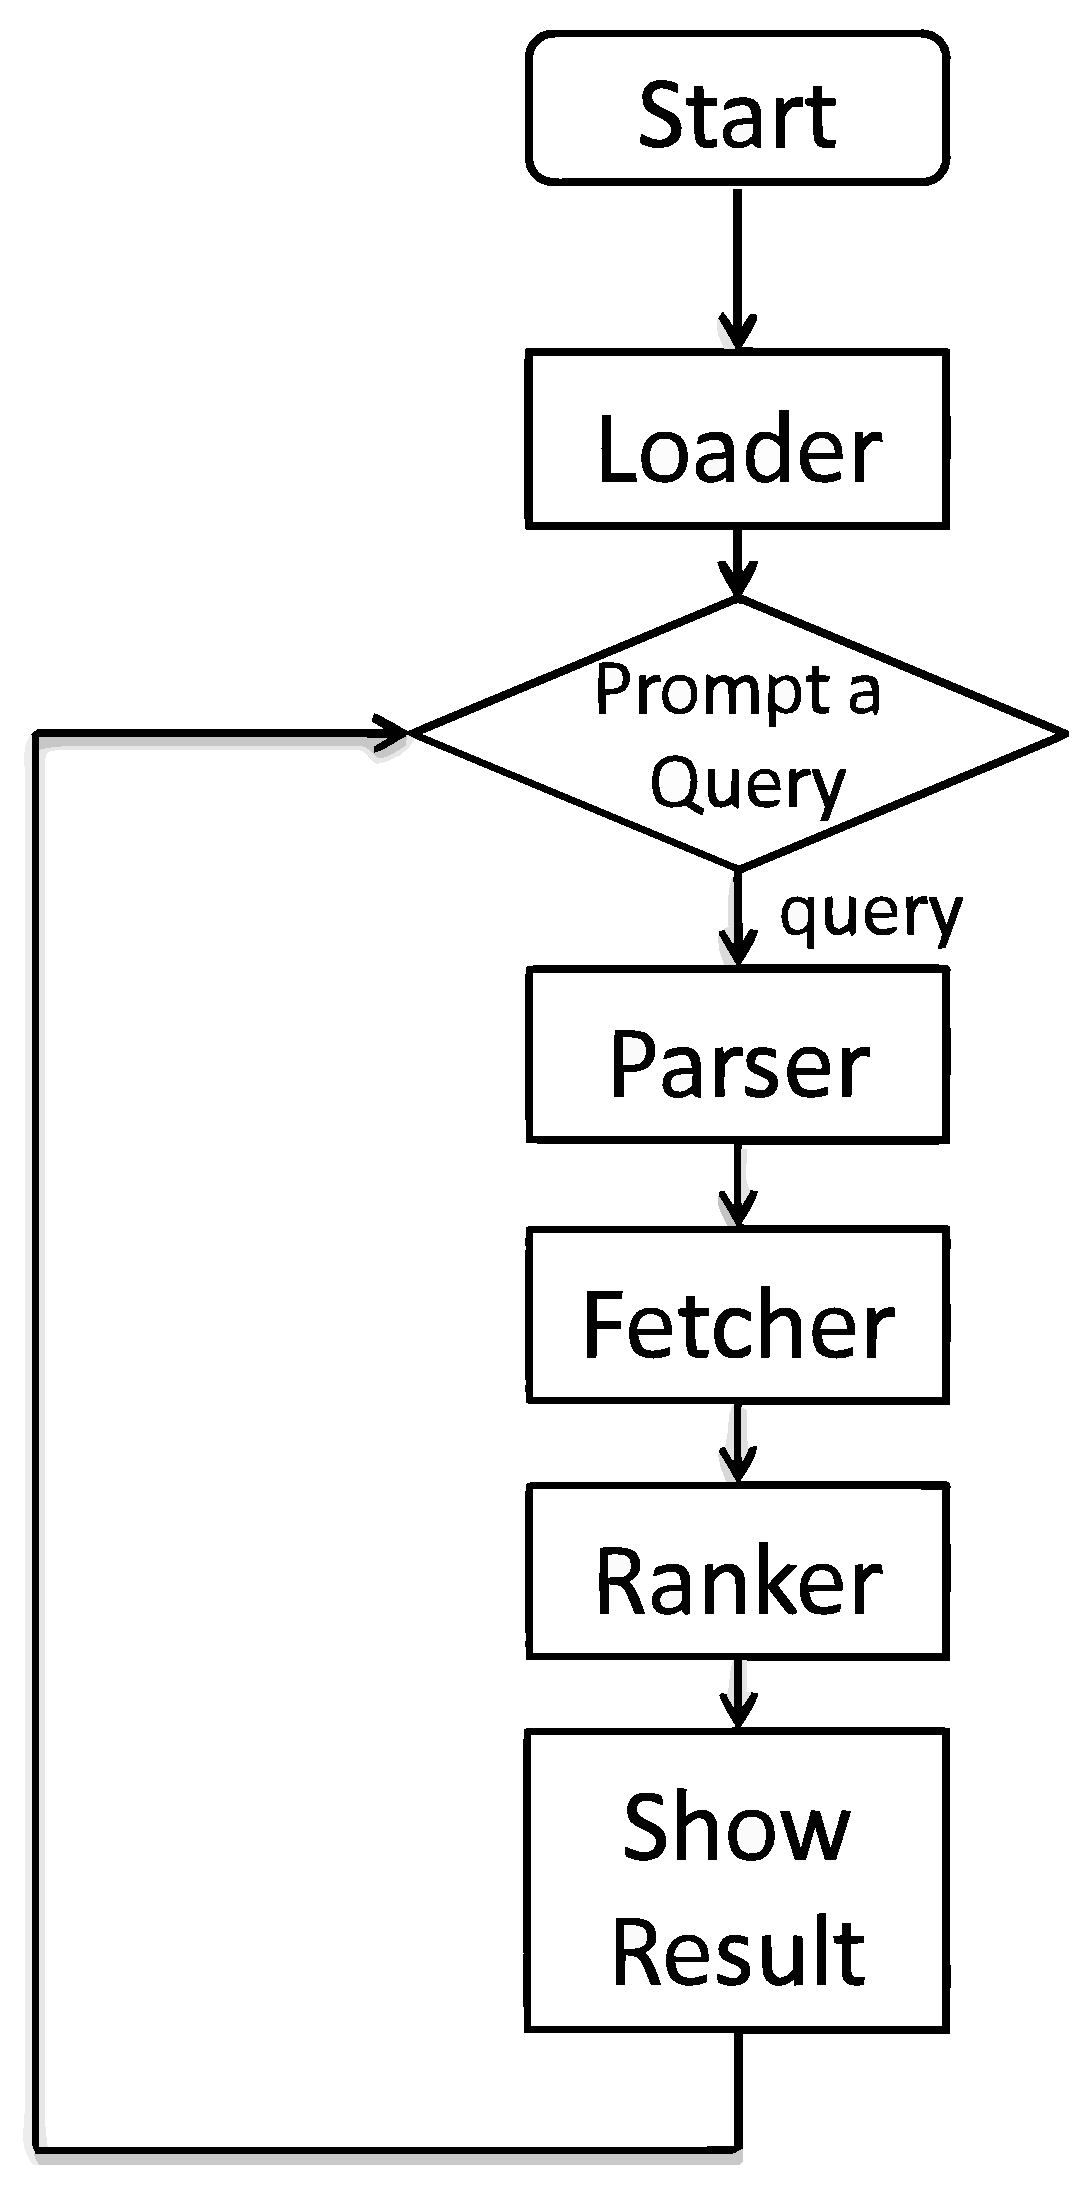
\includegraphics[scale=0.2]{images/system}
  \caption{Overall Structure of Runtime System}
  \label{fig:system}
\end{figure}

\subsection{Loader}
This module is started right after runtime system begins. \textbf{Loader} plays a role as a data provider. It loads necessary data into memory and caches regularly used disk-stored data. Such data includes but not limited:

\begin{itemize}
  \item Instance list and Concept list from Probase.
  \item All historical queries in search log.
  \item Aggregation file.
\end{itemize}

\subsection{Parser}
This module receives a string query from user and uses information from \textbf{Loader} to parse the query into a sequence of Probase concepts and keywords. The complete algorithm is listed in Algorithm \ref{alg:parse}.

\begin{algorithm}
\caption{Parsing Function}
\label{alg:parse}
\begin{algorithmic} [1]
  \REQUIRE a query Q;
  \ENSURE a sequence of concepts and keywords SEQ;

  \STATE $SEQ \Leftarrow PostagParser(Q)$ \\
  \COMMENT {use a postag parser to do word-splitting and postaging}
  \STATE $L \Leftarrow LengthOf(SEQ)$
  \FOR {$max = L$ to $1$}
    \FOR {$i = 0$ to $L - max$}
      \IF {no concept from $SEQ[i]$ to $SEQ[i+max]$}
        \STATE $Test \Leftarrow$ Link $SEQ[i]$ to $SEQ[i+max]$
      \ENDIF
      \IF {$Test$ is a concept}
        \STATE $SEQ[i] \Leftarrow Test$
        \STATE Mark $SEQ[i]$ as a concept
        \STATE Remove $SEQ[i+1]$ to $SEQ[i+max]$
        \STATE $L \Leftarrow L - max + 1$
      \ENDIF
    \ENDFOR
  \ENDFOR
  \RETURN $SEQ$
\end{algorithmic}
\end{algorithm}

\subsubsection{Time Complexity Analysis}
In the worst case, there are no concepts in the query. \textbf{Parser} has to test
\[(1+2+ \cdots +m) = \frac {m \times (m+1)} {2}\] times
, where $m$ is number of words in the query. Besides, the cost of each test is $O(1)$ because the test is based on hash algorithm. In total, the overall time complexity of \textbf{Parser} is $O(m^2)$.

\subsection{Fetcher}
This module receives concept list from \textbf{Parser} and get aggregation list of each concept from \textbf{Loader}. And then, Fetcher does an intersection work to these lists and turns one list of historical queries to next module. The complete algorithm is listed in Algorithm \ref{alg:fetch}.

\begin{algorithm}
\caption{Fetching Function}
\label{alg:fetch}
\begin{algorithmic} [1]
  \REQUIRE a sequence of concepts and keywords $SEQ$
  \ENSURE an intersected aggregation list of concepts

  \STATE $LIST \Leftarrow \varnothing$

  \FOR {$i = 1$ to $LengthOf(SEQ)$}
    \IF {$SEQ[i]$ is a concept}
      \STATE $C_i \Leftarrow$ fetch aggregation list of $SEQ[i]$ from \textbf{Loader}
      \STATE add $C_i$ to $LIST$
    \ENDIF
  \ENDFOR
  \RETURN $\bigcap_{i=1}^{\infty} C_i$, $C_i \in LIST$
\end{algorithmic}
\end{algorithm}

\subsubsection{Time Complexity Analysis}
The routine of \textbf{Fetcher} is divided into two parts - fetching historical query list from aggregation file and intersecting the fetched lists.

For fetching part, like we have done in Section \ref{sec:spaceAnalysis}, assume three parameters - $I_{hq}$, $C_I$ and $n$.

\subsection{Ranker}
